\newpage

\section{Divide and Conquer}
Recursively:
\begin{enumerate}
    \item \textbf{Divide} the problem into a number of sub problems
    \item \textbf{Conquer} the sub problems by solving them recursively
    \item \textbf{Combine} the solutions to the sub problems into the solution for the original problem
\end{enumerate}
General recurrence: 
\begin{align*}
    T(N)=aT(N/b)+f(N)
\end{align*}

\subsection{Closest Points Problem}
Given $N$ points in a plane.  Find the closest pair of points.  (If two points have the same position, then that pair is the closest with distance 0.)


Let $a=b=2, f(N)=cN, k=\log_2 N$
\begin{align*}
    T(N)&=2T(N/2)+cN\\
    &=2^kT(N/2^k)+kcN\\
    &=N+cN\log N=O(N\log N)
\end{align*}




\subsection{Methods for solving recurrences}
\subsubsection{Substitution method}
Guess, then prove by induction. Always assume $T( n ) = \Theta ( 1 )$ for small $n$.
\begin{itemize}
    \item [Example:] $T(N)=2T(\lfloor N/2 \rfloor)+N$
    \item [Guess:] $T(N)=O(N\log N)$
    \item [Proof:] Assume it's true for all $n<N$, in particular for $m=\lfloor N/2 \rfloor$.
    \subitem Then there exists a constant $c>0$ so that
    \begin{align*}
        T(\lfloor N/2 \rfloor)\le c\lfloor N/2 \rfloor\log\lfloor N/2 \rfloor
    \end{align*}
    \subitem Substituting into the recurrence:
    \begin{align*}
        T(N)&=2T(\lfloor N/2 \rfloor)+N\\
        &\le 2c\lfloor N/2 \rfloor\log \lfloor N/2 \rfloor+N\\
        &\le cN(\log N-\log 2)+N\\
        &\le cN\log N \text{ for }c\ge 1
    \end{align*}
\end{itemize}
Must prove the exact form. (数学归纳的结果需要和假设一致)

\subsubsection{Recursion-tree method}
Example: $T(N)=3T(N/4)+\Theta (N^2)$
\begin{figure}[!htb]
    \centering
    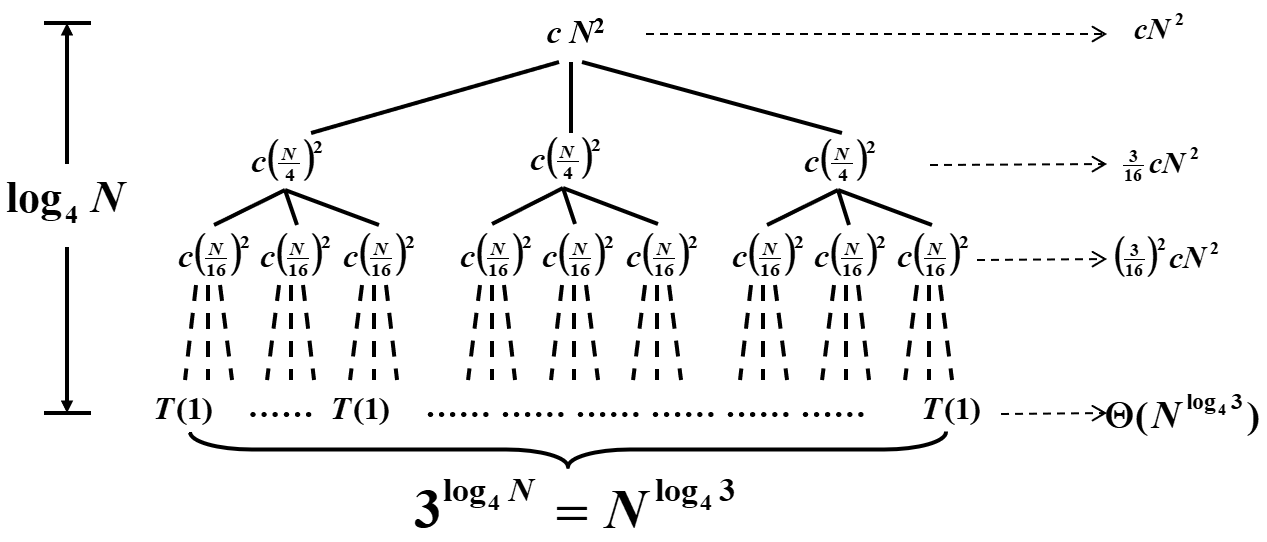
\includegraphics[width=0.42\textwidth]{ADS7/Recursion-tree method}
    \caption{Recursion-tree method}
\end{figure}

\begin{align*}
    T(N)&=\sum_{i=0}^{\log_4 N -1}\left( \frac{3}{16} \right)^i cN^2+\Theta(N^{\log_4 3})\\
    &<\sum_{i=0}^\infty \left( \frac{3}{16} \right)^i cN^2+\Theta(N^{\log_4 3})\\
    &=\frac{cN^2}{1-3/16}+\Theta(N^{\log_4 3})\\
    &=O(N^2)
\end{align*}

仅猜测, 需要用法一进行证明. 

\subsubsection{Master method}
\begin{theorem}[Master method I]\quad 

    Let $a\ge 1$ and $b> 1$ be constants, let $f(N)$ be a function, and let $T(N)$ be defined on the nonnegative integers the recurrence $T(N)=aT(N/b)+f(N)$. Then
    \begin{enumerate}\small
        \item If $\exists\ \epsilon>0,\ f(N)=O(N^{\log_b a-\epsilon})$, then $T(N)=\Theta (N^{\log_b a})$.
        \item If $f(N)=\Theta(N^{\log_b a})$, then $T(N)=\Theta(N^{\log_b a}\log N)$. 
        \item If $\exists\ \epsilon>0,\ f(N)=\Omega(N^{\log_b a+\epsilon})$, and if $\exists\ n>0, N>n$, $\exists\ c<1,\ af(N/b)<cf(N)$ (regularity condition), then $T(N)=\Theta(f(N))$.
    \end{enumerate}
\end{theorem}

%  Read Ch.4 of “Introduction to Algorithms” for the rest of the proof.

\begin{theorem}[Master method II]\quad 

    The recurrence $T(N)=aT(N/b)+f(N)$ can be solved as follows: 
    \begin{enumerate}\small
        \item If $\exists\ \kappa<1,\ af(N/b)=\kappa f(N)$, then $T(N)=\Theta(f(N))$. 
        \item If $\exists\ K>1,\ af(N/b)=Kf(N)$, then $T(N)=\Theta(N^{\log_b a})$. 
        \item If $af(N/b)=f(N)$, then $T(N)=\Theta(f(N)\log_b N)$. 
    \end{enumerate}
\end{theorem}

\begin{theorem}[Master method III]\quad

    The solution to the equation 
    \begin{align*}
        T(N)=aT(N/b)+\Theta(N^k\log^p N)
    \end{align*}
    where $a\ge 1, b>1, p\ge 0$ is 
    \begin{align*}
        T(N)=\left\{ \begin{array}[c]{ll}
            O(N^{\log_b a}) & \text{if }a>b^k \\
            O(N^k\log^{p+1}N)&\text{if }a=b^k\\
            O(N^k\log^p N)&\text{if }a<b^k
        \end{array} \right.
    \end{align*}
    
\end{theorem}